\section{复现结果}
\noindent 本次复现使用的环境如下所示

\scalebox{0.8}{\lstinputlisting[language=bash, breaklines=false]{codes/neofetch.txt}}
\scalebox{0.9}{\lstinputlisting[language=bash, breaklines=false]{codes/nvidia-smi.txt}}
\lstinputlisting[language=bash]{codes/nvcc.txt}
\lstinputlisting[language=bash]{codes/conda.txt}
\lstinputlisting[language=bash]{codes/python.txt}


在原本的GEM模型上, 我们经过大概8小时的运行, 得到如下的复现结果.
\begin{figure}[H]
    \centering
    \begin{subfigure}{0.45\textwidth}{
        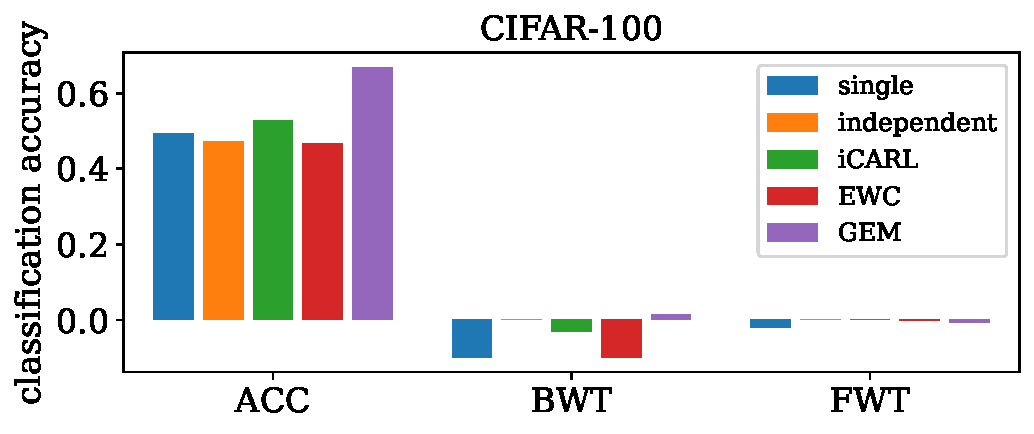
\includegraphics[width=\linewidth]{barplot_cifar100.pdf}
        \caption{Bar plot of accuracy on CIFAR-100}
        \label{fig:barplot}
    }
    \end{subfigure}
    \begin{subfigure}{0.45\textwidth}{
        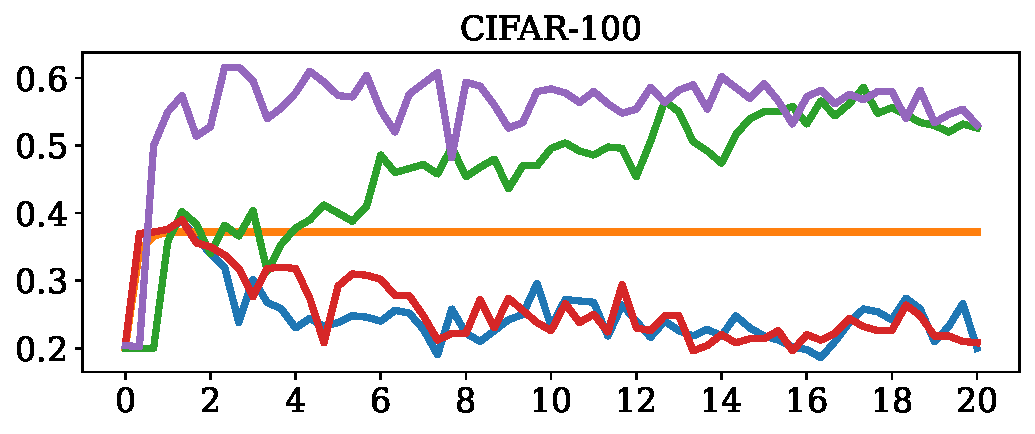
\includegraphics[width=\linewidth]{evoplot_cifar100.pdf}
        \caption{Evo plot of accuracy on CIFAR-100}
        \label{fig:evoplot}
    }
    \end{subfigure}
\end{figure}


将GEM模型嵌入到LibContinual中, 我们得到的复现结果如附录\ref{sec:appendix-log}所示. 可以发现我们的复现效果基本相当于论文中的效果.